% Appendix 3: Projections of a 3D parametric curve onto coordinate planes
\begingroup
\small
\setlength{\parskip}{0.4em}

\noindent\fbox{%
\begin{minipage}{0.97\textwidth}
\textit{\textbf{Enrichment.} Orthogonal projections onto coordinate planes are a core sketching strategy for 3D parametric curves. This example uses the circular helix from part~(a) of Problem~2.21 (\emph{Sketching 3D Parametric Curves}).}
\end{minipage}}

\vspace{0.5em}
\noindent\textbf{Example curve.}
\[
\mathbf{r}(t) = (2\sin t)\mathbf{i} + (2\cos t)\mathbf{j} + \frac{t}{\pi}\mathbf{k},
\qquad 0 \le t \le 4\pi.
\]
Equivalently, $x(t)=2\sin t$, $y(t)=2\cos t$, and $z(t)=t/\pi$.

\vspace{0.3em}
\noindent\textbf{The curve in 3D.}
\begin{center}
\tdplotsetmaincoords{70}{120}
\begin{tikzpicture}[tdplot_main_coords, scale=0.72]
  \draw[thin,->] (0,0,0) -- (3.2,0,0) node[anchor=north east]{\scriptsize $x$};
  \draw[thin,->] (0,0,0) -- (0,3.2,0) node[anchor=north west]{\scriptsize $y$};
  \draw[thin,->] (0,0,0) -- (0,0,4.8) node[anchor=south]{\scriptsize $z$};
  \draw[dashed,gray!50] (0,0,0) -- (-2.8,0,0);
  \draw[dashed,gray!50] (0,0,0) -- (0,-2.8,0);

  % Coordinate planes (light shading for projection context)
  \fill[blue!6,opacity=0.35] (-2.5,-2.5,0) -- (2.5,-2.5,0) -- (2.5,2.5,0) -- (-2.5,2.5,0) -- cycle;
  \fill[red!6,opacity=0.25] (0,-2.5,0) -- (0,2.5,0) -- (0,2.5,4.2) -- (0,-2.5,4.2) -- cycle;
  \fill[green!6,opacity=0.25] (-2.5,0,0) -- (2.5,0,0) -- (2.5,0,4.2) -- (-2.5,0,4.2) -- cycle;

  \draw[thick,blue,domain=0:4*pi,samples=160,smooth]
    plot ({2*sin(\x r)},{2*cos(\x r)},{\x/pi});

  \fill[blue!70!black] (0,2,0) circle (1.8pt);
  \node[anchor=west,font=\scriptsize] at (0.08,2,0) {$(0,2,0)$};
  \fill[blue!70!black] (0,2,4) circle (1.8pt);
  \node[anchor=west,font=\scriptsize] at (0.08,2,4) {$(0,2,4)$};
\end{tikzpicture}
\end{center}

\noindent\textbf{Orthogonal projections onto the coordinate planes.}
Each projection keeps two components and sets the third to zero---the ``shadow'' of the curve when viewed along the missing axis.

\vspace{0.25em}
\noindent
\begin{minipage}[t]{0.32\textwidth}
\centering
\textbf{Projection onto the $xy$-plane}\\[0.15em]
\scriptsize Drop $z$: $(x,y)=(2\sin t,\,2\cos t)$\\[0.25em]
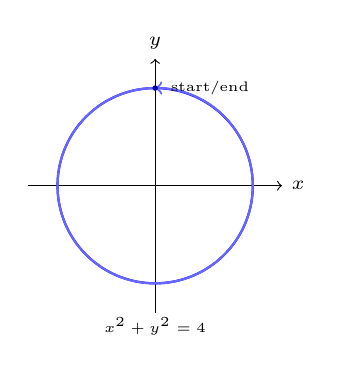
\begin{tikzpicture}[scale=0.62,baseline=(current bounding box.center)]
  \draw[thin,->] (-2.6,0) -- (2.6,0) node[right]{\scriptsize $x$};
  \draw[thin,->] (0,-2.6) -- (0,2.6) node[above]{\scriptsize $y$};
  \draw[thick,blue,domain=0:360,samples=100,smooth]
    plot ({2*sin(\x)},{2*cos(\x)});
  \draw[->,thick,blue!60] (0,2) arc (90:450:2);
  \fill[blue!70!black] (0,2) circle (1.6pt);
  \node[font=\tiny,anchor=west] at (0.12,2) {start/end};
  \node[font=\tiny,anchor=north] at (0,-2.5) {$x^2+y^2=4$};
\end{tikzpicture}\\[0.15em]
\scriptsize Circle of radius~$2$, traversed \textbf{twice} as $t$ runs from $0$ to $4\pi$.
\end{minipage}\hfill
\begin{minipage}[t]{0.32\textwidth}
\centering
\textbf{Projection onto the $yz$-plane}\\[0.15em]
\scriptsize Drop $x$: $(y,z)=(2\cos t,\,t/\pi)$\\[0.25em]
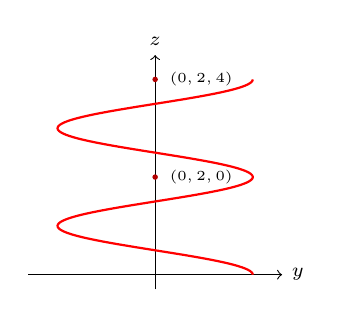
\begin{tikzpicture}[scale=0.62,baseline=(current bounding box.center)]
  \draw[thin,->] (-2.6,0) -- (2.6,0) node[right]{\scriptsize $y$};
  \draw[thin,->] (0,-0.3) -- (0,4.5) node[above]{\scriptsize $z$};
  \draw[thick,red,domain=0:4*pi,samples=160,smooth]
    plot ({2*cos(\x r)},{(\x)/pi});
  \fill[red!70!black] (0,2) circle (1.6pt);
  \fill[red!70!black] (0,4) circle (1.6pt);
  \node[font=\tiny,anchor=west] at (0.1,2) {$(0,2,0)$};
  \node[font=\tiny,anchor=west] at (0.1,4) {$(0,2,4)$};
\end{tikzpicture}\\[0.15em]
\scriptsize Sinusoidal trace: $y=2\cos(\pi z)$ for $0\le z\le 4$ (two full periods).
\end{minipage}\hfill
\begin{minipage}[t]{0.32\textwidth}
\centering
\textbf{Projection onto the $xz$-plane}\\[0.15em]
\scriptsize Drop $y$: $(x,z)=(2\sin t,\,t/\pi)$\\[0.25em]
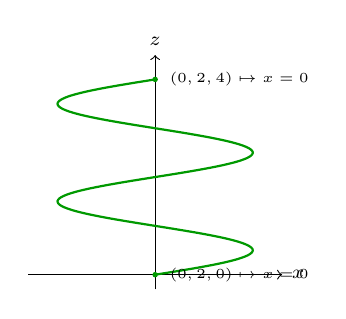
\begin{tikzpicture}[scale=0.62,baseline=(current bounding box.center)]
  \draw[thin,->] (-2.6,0) -- (2.6,0) node[right]{\scriptsize $x$};
  \draw[thin,->] (0,-0.3) -- (0,4.5) node[above]{\scriptsize $z$};
  \draw[thick,green!60!black,domain=0:4*pi,samples=160,smooth]
    plot ({2*sin(\x r)},{(\x)/pi});
  \fill[green!60!black] (0,0) circle (1.6pt);
  \fill[green!60!black] (0,4) circle (1.6pt);
  \node[font=\tiny,anchor=west] at (0.1,0) {$(0,2,0)\mapsto x=0$};
  \node[font=\tiny,anchor=west] at (0.1,4) {$(0,2,4)\mapsto x=0$};
\end{tikzpicture}\\[0.15em]
\scriptsize Sinusoidal trace: $x=2\sin(\pi z)$ for $0\le z\le 4$ (two full periods).
\end{minipage}

\vspace{0.5em}
\noindent\textbf{What we find, and how to read the projections.}

\begin{itemize}[leftmargin=*,itemsep=0.25em]
  \item \textbf{$xy$-projection (view from above, along $\mathbf{k}$).}
  Only the $\mathbf{i}$ and $\mathbf{j}$ components matter. Here $x^2+y^2=4$, so the shadow is a circle of radius~$2$. Because $t$ ranges over $4\pi$, the particle winds around this circle \emph{twice} while rising in~$z$. The projection alone does not show the vertical motion---it only reveals that the helix sits on a vertical cylinder of radius~$2$.

  \item \textbf{$yz$- and $xz$-projections (side views).}
  Each pairs one horizontal coordinate with height. Substituting $t=\pi z$ gives $y=2\cos(\pi z)$ and $x=2\sin(\pi z)$ on $0\le z\le 4$. Both shadows are sinusoidal waves with amplitude~$2$ and two complete periods---matching the two revolutions of the helix.

  \item \textbf{Reconstructing the 3D curve.}
  Read the curve component-wise: circular motion in the $xy$-plane combined with steady linear increase in~$z$. The start point is $\mathbf{r}(0)=(0,2,0)$ and the end point is $\mathbf{r}(4\pi)=(0,2,4)$---both visible on every projection at $z=0$ and $z=4$ with $x=0$.

  \item \textbf{Sketching strategy (HSC and beyond).}
  When a 3D parametric equation looks unfamiliar, project onto each coordinate plane first. Each projection is a 2D curve you can sketch using familiar methods. Then combine the information: if the $xy$-shadow is a circle and $z$ grows steadily, expect a helix; if two horizontal coordinates match (as in part~(b) of the same problem), the curve is confined to a plane.
\end{itemize}

\endgroup
